%!TEX root = index.tex
\section[Introdução]{Introdução}


\begin{frame}{Introdução}{Importância econômica}
\begin{columns}[b] % The "c" option specifies centered vertical alignment while the "t" option is used for top vertical alignment

\column{.5\textwidth} %
\begin{figure}[ht]
    \begin{center}
    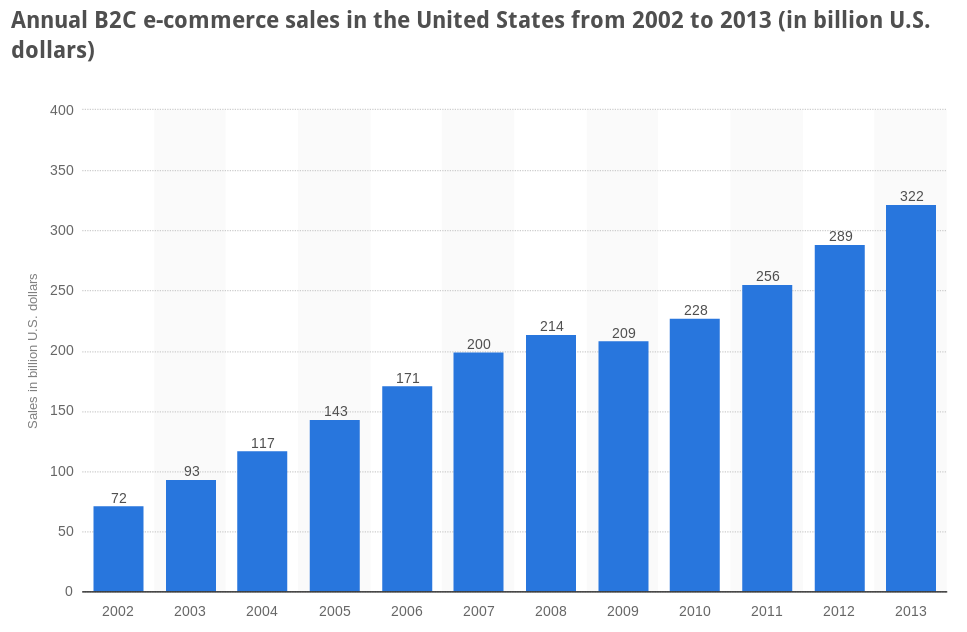
\includegraphics[width=1\textwidth]{img/sales-ecommerce}\caption{Vendas de varejo atribuídas a lojas online nos EUA \cite{sales-ecommerce}}
    \end{center}
\end{figure}

\column{.5\textwidth} % 

\begin{figure}[ht]
    \begin{center}
    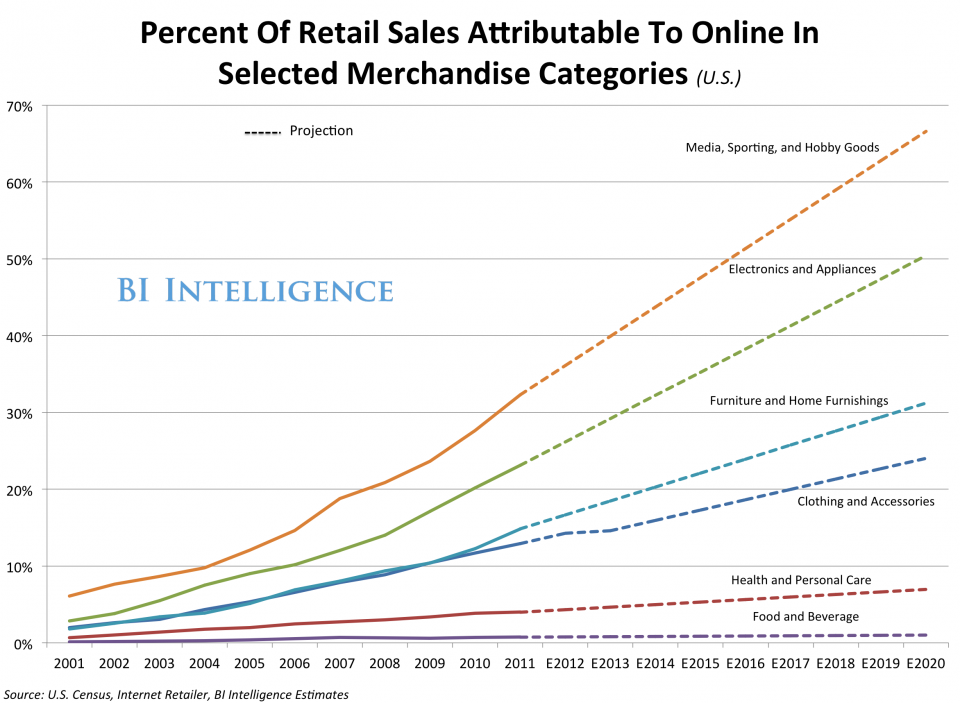
\includegraphics[width=1\textwidth]{img/crescimento-ecommerce}\caption{Percentual de vendas de varejo atribuídas a lojas online nos EUA por categoria \cite{crescimento-ecommerce}}
    \end{center}
\end{figure}



\end{columns}

\end{frame}


\begin{frame}{Introdução}{Aplicação}
\begin{columns}[c]

\column{.5\textwidth} % Left column and width

\begin{figure}[ht]
    \begin{center}
    
\includegraphics[height=30px]{img/facebook}

    Relações de amizade
    \end{center}
\end{figure}

\column{.5\textwidth} % Right column and width

\begin{figure}[ht]
    \begin{center}
    \includegraphics[height=30px]{../img/lastfm}

    Músicas
    \end{center}
\end{figure}
\end{columns}
\begin{columns}[b]

\column{.3333\textwidth}

\begin{figure}[ht]
    \begin{center}
    
\includegraphics[height=30px]{img/amazon}

    Livros \textbf{35 \%} \\
    \cite{amazon35}
    \end{center}
\end{figure}

\column{.3333\textwidth}
\begin{figure}[ht]
    \begin{center}
    
\includegraphics[height=23px]{img/google-news}

    Notícias \textbf{38 \%} \\
    \cite{das2007google}
    \end{center}
\end{figure}

\column{.3333\textwidth}
\begin{figure}[ht]
    \begin{center}
    \includegraphics[height=30px]{../img/netflix}

    Filmes \textbf{75 \%} \\
    \cite{netflix75}
    \end{center}
\end{figure}
\end{columns}
\end{frame}




%\begin{frame}{Introdução}{O que são Sistemas de Recomendação?}
%\begin{block}{Definição}
%``São ferramentas e técnicas de software destinadas a prover sugestões de itens para usuários'' \cite{ricci2011introduction-chap1}
%\end{block}
%
%\begin{block}{Etapas principais}
%\begin{itemize}
%    \item Aquisição dos dados de entrada
%    \item Determinação das recomendações
%    \item Apresentação dos resultados ao usuário
%\end{itemize}
%\end{block}
%\end{frame}
